\begin{figure*}[t]
\centering
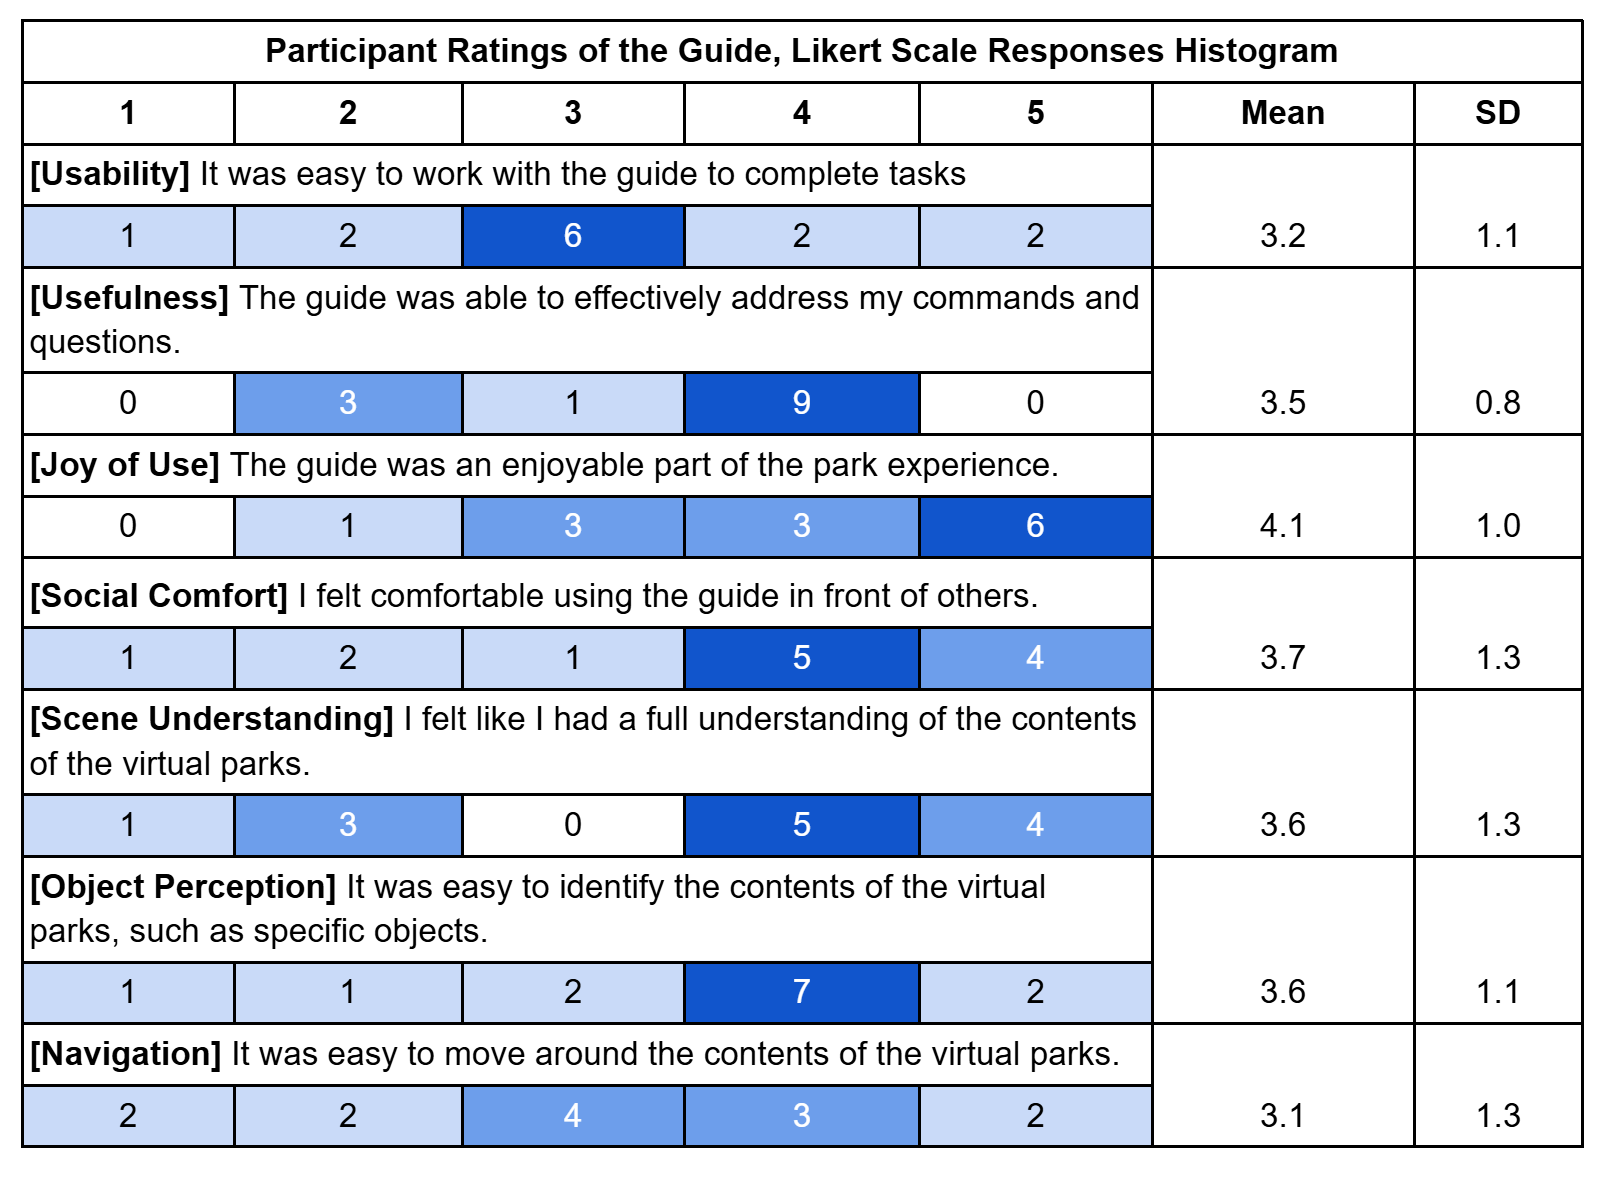
\includegraphics[width=350pt]{likert_responses.png}
\caption{\label{fig: Likert Guide Ratings} Likert scale responses from participants rating the guide, collected after participants experienced both parks and guide personas. Scores were given on a scale of 1 to 5, where 1 = strongly disagree, 2 = disagree, 3 = neither agree nor disagree, 4 = agree, and 5 = strongly agree. Note: In the statement on Social Comfort, “others” refers to the confederates participants met during the study. We only include scores from thirteen participants who used the guide.
}
\Description{A histogram containing the Likert-scale response data from participants rating the guide on various qualities. The scale runs from 1 to 5, with numbers in columns below depicting how many responses from participants fell under each number on the scale for a given statement and factor. They are colored in various shades of blue, with the darker colors representing more responses falling under a particular number on the scale and the lighter colors representing fewer.

For the statement: [Usability] It was easy to work with the guide to complete tasks.
The histogram reports 1 user responded 1, 2 users responded 2, 6 users responded 3, 2 users responded 4, and 2 users responded 5. The mean is 3.2, standard deviation 1.1.

For the statement: [Usefulness] The guide was able to effectively address my commands and questions.
The histogram reports 0 users responded 1, 3 users responded 1, 1 user responded 3, 9 users responded 4, and 0 users responded 5. The mean is 3.5, standard deviation 0.8. 

For the statement: [Joy of Use] The guide was an enjoyable part of the park experience.
The histogram reports 0 users responded 1, 1 user responded 2, 3 users responded 3, 3 users responded 4, and 6 users responded 5. The mean is 4.1, standard deviation 1.0. 

For the statement: [Social Comfort] I felt comfortable using the guide in front of others.
The histogram reports 1 user responded 1, 2 users responded 2, 1 user responded 3, 5 users responded 4, and 4 users responded 5. The mean is 3.7, standard deviation 1.3. 

For the statement: [Scene Understanding] I felt like I had a full understanding of the contents of the virtual parks.
The histogram reports 1 user responded 1, 3 users responded 2, 0 users responded 3, 5 users responded 4, and 4 users responded 5. The mean is 3.6, standard deviation 1.1. 

For the statement: [Object Perception] It was easy to identify the contents of the virtual parks, such as specific objects.
The histogram reports 1 user responded 1, 1 user responded 2, 2 users responded 3, 7 users responded 4, and 2 users responded 5. The mean is 3.6, standard deviation 1.1. 

For the statement: [Navigation] It was easy to move around the contents of the virtual parks.
The histogram reports 2 users responded 1, 2 users responded 2, 4 users responded 3, 3 users responded 4, and 2 users responded 5. The mean is 3.1, standard deviation 1.3. 

}
\end{figure*}